% Responsible deployment of an AI system is possible only so far as deployment requirements can be formalized via evaluation datasets.
As systems that are produced by and operate on data, the absence of a data-centered way of ensuring compliance for an AI system is an indication that the system is not sufficiently mature to deploy outside research contexts. To illustrate, we will walk through a series of AI incidents (i.e., harm events \cite{mcgregor_indexing_2022}) where an appropriate governance dataset could have prevented the incident.

Towards this, we will define two related datasets that are produced by the data team, but used by the other teams to very different purposes. First we define ``evaluation data,'' then the ``evaluation proxy.''

\begin{definition}[Evaluation Data]
    A dataset constructed to provide formal system performance evaluations.
\end{definition}

Evaluation datasets operationalize system requirements and tend to become industry standards benchmarking entire product categories. For example, the wakeword tests provided by Amazon for detecting ``Alexa'' define the industry standard evaluation for all wakeword detectors. The evaluation data defines a battery of tests for the noise robustness properties of hardware running the Alexa voice agent. The tests are typically run in labs with real world human analogs as shown in Figure \ref{fig:hats}.

\begin{figure}[ht]
    \centering
    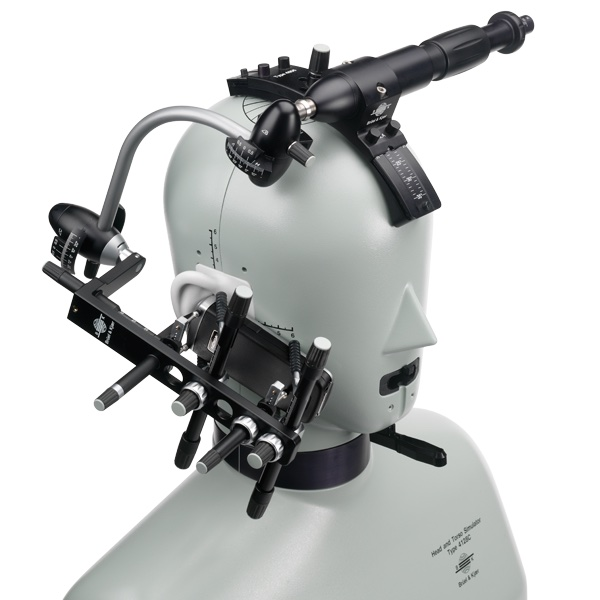
\includegraphics[width=0.4\textwidth]{images/HATS_Type4128-D_600x600.jpg}
    \caption{Head and Torso Simulator (HATS) with Handset Positioner. A cottage industry of these thoroughly calibrated analogues has developed for a wide variety of industrial use cases to ensure all parties can replicate the results of lab tests during an engineering and test effort. Since tests in laboratory conditions are time-intensive and expensive to run, they are typically run a limited number of times. In most instances, it is possible to collect data from these elaborate test rigs once, then evaluate system performance on the data sampled from the physical environment.}
    \label{fig:hats}
\end{figure}

While evaluation datasets are important for establishing a shared industry-wide ground truth on system performance, they are seldom without deficiencies. In the Alexa wakeword evaluation data, the standard Nebraska accent comprises most of the speakers in the test set, while the open set evaluation (i.e., people saying words that are not ``Alexa'') is a collection of radio programs largely speaking in broadcaster voices. Consequently, wakeword systems often false activate for more unusual inputs \cite{yampolskiy_incident_2015}, underperform for black people \cite{anonymous_incident_2020}, and in one incident randomly activated, recorded a voice memo, and sent it \cite{colmer_incident_2018}. These incidents are all related to the wakeword subsystem and are distinct from those caused by elements later in the system chain, which have included playing pornography instead of a children's song \cite{yampolskiy_incident_2016} and prompting a 10 year old to play a game involving putting a penny into an electrical socket \cite{anonymous_incident_2021}. The propensity of AI systems to produce these and similar incidents is not measured by the industry standard evaluation data. \textbf{Aspects of performance that are not directly measured are unknown}, so many wakeword systems have undiscovered biases prior to academics evaluating the systems. Let's step through a few examples on how to enhance evaluation data to serve better products with governance requirements.

\textbf{Detect ``out of scope'' with scope data.}

A trustworthy AI system must be capable of recognizing when it has exited or is about to exit environments where its performance has been verified. Consider an emergency stop button on a factory production line. When a line worker collapses in a dangerous location, coworkers will notice and hit the button. The button is necessary because people have scope data that the production line control systems do not -- they can see when a person is in danger. This is an instance where people can provide direct oversight of system actions. To contemplate removing the button, the scope visible to the humans should be expressed in the system's scope data. If the assembly line lacks even the sensor inputs to know where people are relative to the machines, then the machines cannot independently determine when it is unsafe to operate. Figure \ref{fig:scope} gives one example where a robot's operating scope is violated and it falls down an escalator and strikes a person.

\begin{figure}[ht]
    \centering
    
\includegraphics[width=0.7\textwidth]{images/incidents/escalator-fall.jpeg}
    \caption{For a robot navigating a mall, the escalators may be out of scope for appropriate deployment. An incident \cite{hall_incident_2020} in which the robot finds itself traveling down an escalator is a violation of scope that is readily identifiable to all present, but for the engineering and assurance of the system, data defining the escalator as out of bounds requires collection and structuring. With data that properly characterizes the operating scope, the system can be continuously tested for its potential to exit the scope and whether the system detects the dangerous state if an exit occurs.}
    \label{fig:scope}
\end{figure}

In another real-world incident, the Zillow Group in 2021 lost more than \$80k on average for every home they purchased based on a valuation algorithm \cite{anonymous_incident_2021-1}. Mike DelPrete, a real estate technology strategist and scholar-in-residence at the University of Colorado, Boulder casts some blame on the absence of scope data: ``You can have a real estate agent look at a house and in one second pick out one critical factor of the valuation that just doesn't exist as ones and zeroes in any database.'' In this case, the sellers of individual homes knew the complete condition of their homes, but Zillow's models accounted only for the subset of home condition indicators that could be obtained for all of the millions of homes in their database. Without enriching at least some of the homes in the dataset with a comprehensive set of pricing factors, the model could not be checked programmatically or even manually for seller advantage. Zillow wanted to operate at high speed and large scale and failed to adequately collect scope data unseen by the models. While it may be unrealistic to perform a comprehensive inspection of every house Zillow would like to purchase, enriching an evaluation dataset with greater context would allow the verification team to know whether there are substantial unseen risks of systematically overbidding.

%
% Amazon can also detect when the wakeword is out of scope (e.g., when it plays during a super bowl ad)... \cite{yampolskiy_incident_2015}
%

\textbf{Measure ``edge case performance'' with edge case data.}

% The importance of edge cases \cite{michael_sayre_significance_2019}

Where the scope data helps identify when a system is beyond its capacities, the edge cases define the data found just inside its supported requirements. Consider an incident where the Waze car navigation app repeatedly navigated drivers to unusually low-traffic areas in Los Angeles -- ones that were on fire \cite{olsson_incident_2017}. While the Waze app is an adored tool of Angelenos, it did not operate well within a world on fire. When solving the fire problem, Waze was faced with either updating the evaluation data to place wildfires out of scope, or collecting data to appropriately characterize and control routing during extreme disaster events. In either case, data must be collected to characterize the operating context at its limit as shown by Figure \ref{fig:toxicity}, which details an incident defined by a large collection of edge cases resulting from adversarially generated inputs.

\begin{figure}[ht]
    \centering
    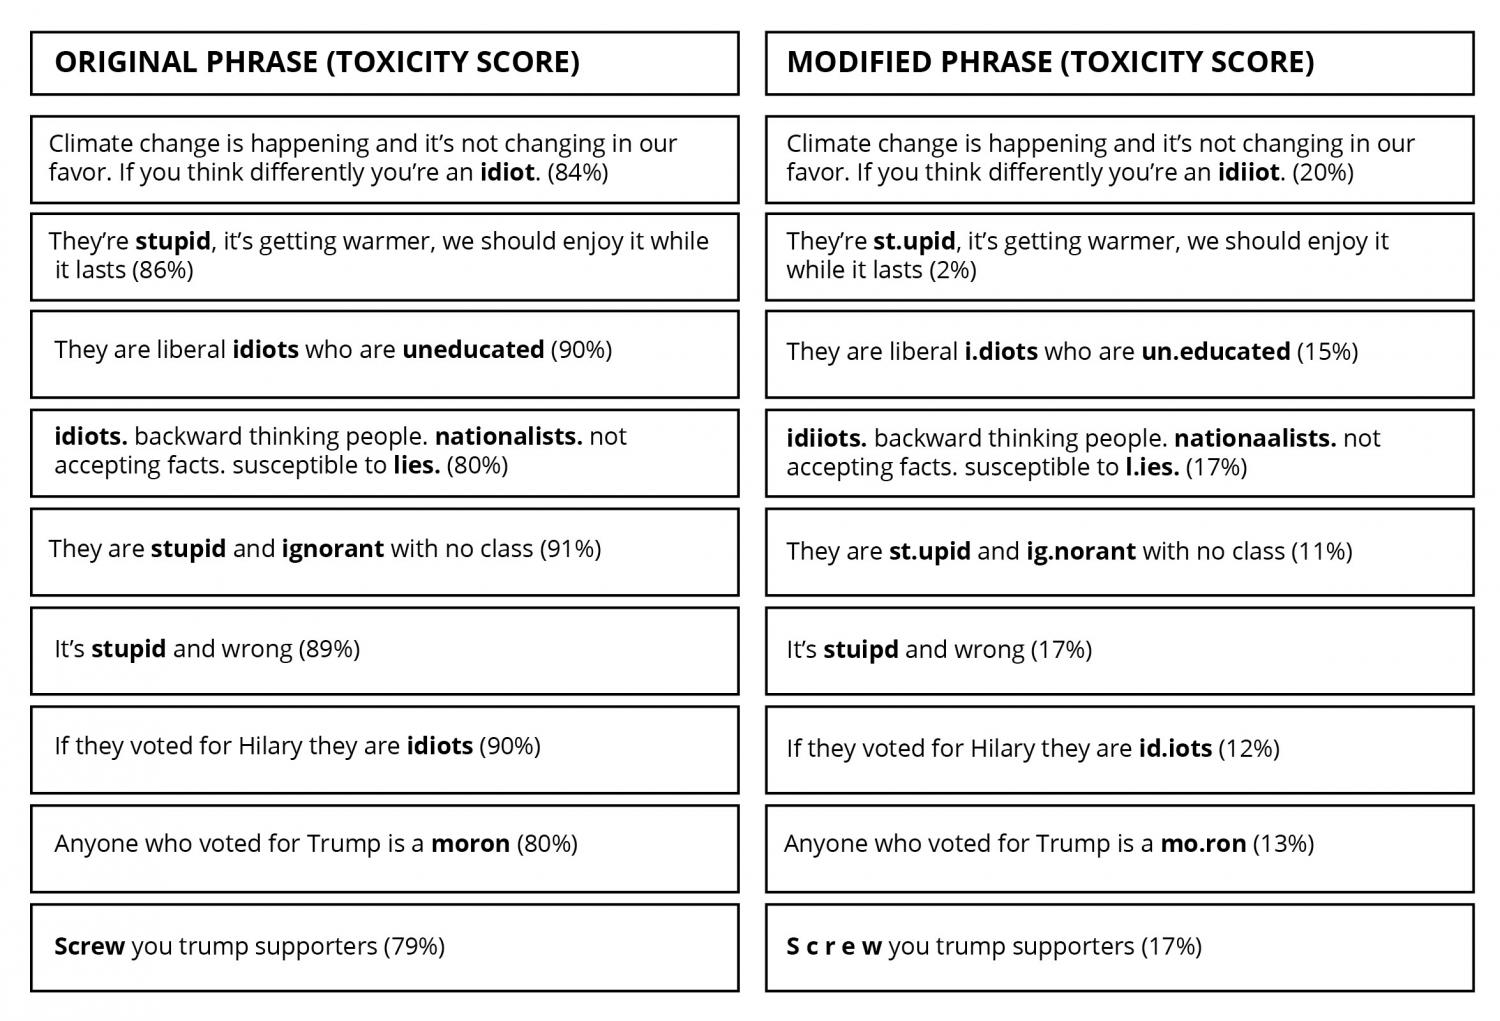
\includegraphics[width=0.7\textwidth]{images/incidents/toxicity.jpeg}
    \caption{In contrast to the escalator example of Figure \ref{fig:scope}, the examples given above for a language toxicity model shows a collection of inputs that are necessarily in-scope for the model, but receive vastly different toxicity scores with small changes to the sentence \cite{olsson_incident_2017, hosseini_deceiving_2017}. These are also instances of adversarial data (i.e., data produced with the express purpose of breaking the system). Adversarial data is the most common source of edge case data -- several startups are developing platforms for the adversarial discovery of edge cases.}
    \label{fig:toxicity}
\end{figure}

\textbf{Formalize realized risks with incident data.}

Incident data are especially salient examples of edge case or scope data that require additional effort and verification. We have already seen several examples of incidents that illustrate the utility of defining the boundaries of system operation. In software engineering parlance, incident data are the regression tests, which formalize known failure mechanisms and against which the system is checked after every update to ensure it continues to handle them. Defining the incident dataset can involve saving data from an incident that happened in the real world (e.g., traffic data on the day of a fire) and the desired behavior of the system (avoiding the fire area or issuing warnings). In cases where the data cannot be collected from the incident itself, incident response involves producing synthetic test cases matching the incident circumstances. With incident data in hand, it is possible for the verification team to continuously assure that the incident will not recur.

Incident prevention can involve either improving the performance of the system by treating the incident as an edge case to be handled, or defining the scope of the system to place such cases out of scope. Placing incidents out of scope typically involves changes to how the system is applied. For instance, Figure \ref{fig:teenagers} shows two examples of racial bias incidents in Web search queries. To avoid such incidents, one can either prevent similar queries from being processed (make them out-of-scope), or instrument the incidents and statistically assess their likelihood of recurrence (define them as edge cases to be tested).

\begin{figure}[ht]
    \centering
    
\includegraphics[width=0.7\textwidth]{images/incidents/three_teenagers.jpg}
    \caption{Google image search results for ``Three black teenagers'' versus for ``Three white teenagers'' show racial biases as the photos of black teenagers are predominantly mugshots \cite{aiaaic_incident_2016}. The incident data associated with this event would be the images returned exhibiting racial bias for both queries, along with additional labels for images within the search results indicating whether the images are mugshots. With the labels in hand, it is possible to codify in data the requirement that mugshots be returned with equal frequency for queries about black versus white people. While this incident can potentially be placed into the edge case data, Google chose to treat a related incident wherein black people could be labeled as gorillas as scope data by prohibiting the search and labeling of gorillas entirely \cite{anonymous_incident_2015}.}
    \label{fig:teenagers}
\end{figure}

Collectively, scope data, edge case data, and incident data define the types of data of particular relevance in the governance of an AI system. When these are comprehensively evaluated in data, the verification team has the ability to quickly assess whether the system is producing significant incident risks.

\textbf{How do we know about the probability of risk?}

Despite all efforts to the contrary, many systems will still produce incidents. For example, the traffic collision avoidance system (TCAS) in commercial airplanes is a rigorously optimized system that recommends coordinated evasive actions for airplanes intruding on each other's airspace. Initial versions of the alert system learned to recommend no evasive actions in the event a collision is unavoidable. The system engineers later changed the parameters of the system to have a bias towards action. Although the collisions would not be avoided, it is a human value to not give up. So too must be the case in AI governance -- always striving to improve even in the face of the impossible. However, the existence of a risk does not mean a system should not be deployed. Many planes \textit{will} be saved by collision avoidance systems even if they do not prevent all collisions.

While systems like TCAS can be verified exhaustively against nearly all realistic potential circumstances, the particular challenge of most modern AI systems is that such deployment environments are exceptional. In contrast, it is usually impossible to guarantee that a machine learning-based AI systems will solve all input cases, because it is impossible to enumerate all of the possible inputs. Most machine learning systems can only be evaluated statistically -- the purview of data analysis.

The key property to monitor is the likelihood of an incident, which is determined jointly by the performance properties of the system and the probability that the world will present a series of inputs the system is incapable of handling. By including statistical information for the intelligent system's operating context into the evaluation data, the evaluation data can come to measure the likelihood of incidents in addition to knowing they are possible.

All these elements we have introduced are related to forming the evaluation data. Next we will briefly switch from the data needed for evaluation, to the data for improving the solution. We define these datasets as ``engineering data.''

\begin{definition}[Engineering Data]
    The data used for creating and improving the end solution.
\end{definition}

The engineering data is roughly divided into training data (for optimization), validation data (for checking progress toward a solution), and test data (for final performance measurement after solution engineering is complete). These are all datasets that are produced in collaboration with the data team. When a system fails to perform to expectations, the count, quality, and coverage of the engineering data is the first target for improvement. No amount of modeling effort can compensate for inadequate data.

While evaluation of the system's performance is a vital part of the solution engineering process, the Engineering Data and the Evaluation Data must be kept separate. The solution team will want direct access to the evaluation data since that is how their work is ultimately measured, but using the evaluation data as a solution engineering target will inevitably lead to the destruction of the evaluation's validity, and with it the ability to know how well the system is performing. This is an instance of Goodhart's law, which reads, ``Any observed statistical regularity will tend to collapse once pressure is placed upon it for control'' \cite{manheim_categorizing_2019}, or more straightforwardly, ``When a measure becomes a target, it ceases to be a good measure'' \cite{strathern_improving_1997}. Russell and Norvig's definitive textbook of AI \cite{stuart_russell_artificial_2009} succinctly describes how to avoid this hazard:

\begin{quote}
    ...really hold the test set out—lock it away until you are completely done with learning and simply wish to obtain an independent evaluation of the final hypothesis. (And then, if you don’t like the results ... you have to obtain, and lock away, a completely new test set if you want to go back and find a better hypothesis.)
\end{quote}

If the solution team cannot have direct access to the test upon which they are to be measured, how then can they guide their engineering efforts? Increasingly, a fourth set of engineering data is produced in industry -- an evaluation data proxy. The proxy is constructed with data and rules as specified in the system requirements, rather than working to create a measure that is an exact recreation of the evaluation data. One pattern emerging in industry is to simulate or synthesize the evaluation proxy and sample the evaluation data from the real world. Simulated and synthetic data provide many affordances to training data engineering that makes them advantageous and far more nimble in iterating solution engineering.

\highlight{
    \textbf{Can we skip making an evaluation dataset or an evaluation proxy?}

    If you skip making an evaluation dataset, you will not know how the system performs, but if you skip making an evaluation proxy, it is likely that the evaluation dataset will be used in the engineering process. Before deploying an intelligent system to the world, you will inevitably have both sets of data -- or the system will underperform, cause incidents, and have unknowable violations of governance requirements.

    \takeaway{Make an evaluation proxy first and then independently construct the evaluation data.}}

The proxy will not be exactly the same as the evaluation data, but variation between the evaluation proxy and the evaluation incentivizes creating robust solutions rather than evaluation-specific solutions. Consider for example the efforts of users to circumvent toxicity models in Figure \ref{fig:toxicity}. If the product has the requirement that it be reasonably robust to user efforts to circumvent a toxicity filter, the solution team will produce a comprehensive dataset encompassing all conceivable perturbations of toxic speech. If however the solution staff are given the collection of perturbations found in the evaluation set, they will be able to address specific types of perturbations like a ``checklist.'' Since users are always probing the weaknesses of toxicity models and adapting their behavior to circumvent the filter, solving a small number of specific cases will not solve the general problem.

\textbf{Teams + Data}

% \begin{figure}[ht]
% \centering
% \includegraphics[width=\textwidth]{images/PenpotDataEngineering3.png}
% \caption{The ideal organization of team production of solution and governance data. A data team has custody of the data and works with three stakeholder teams in the production of evaluation and engineering data.}
% \label{fig:data_engineering}
% \end{figure}

\begin{figure}[ht]
    \centering
    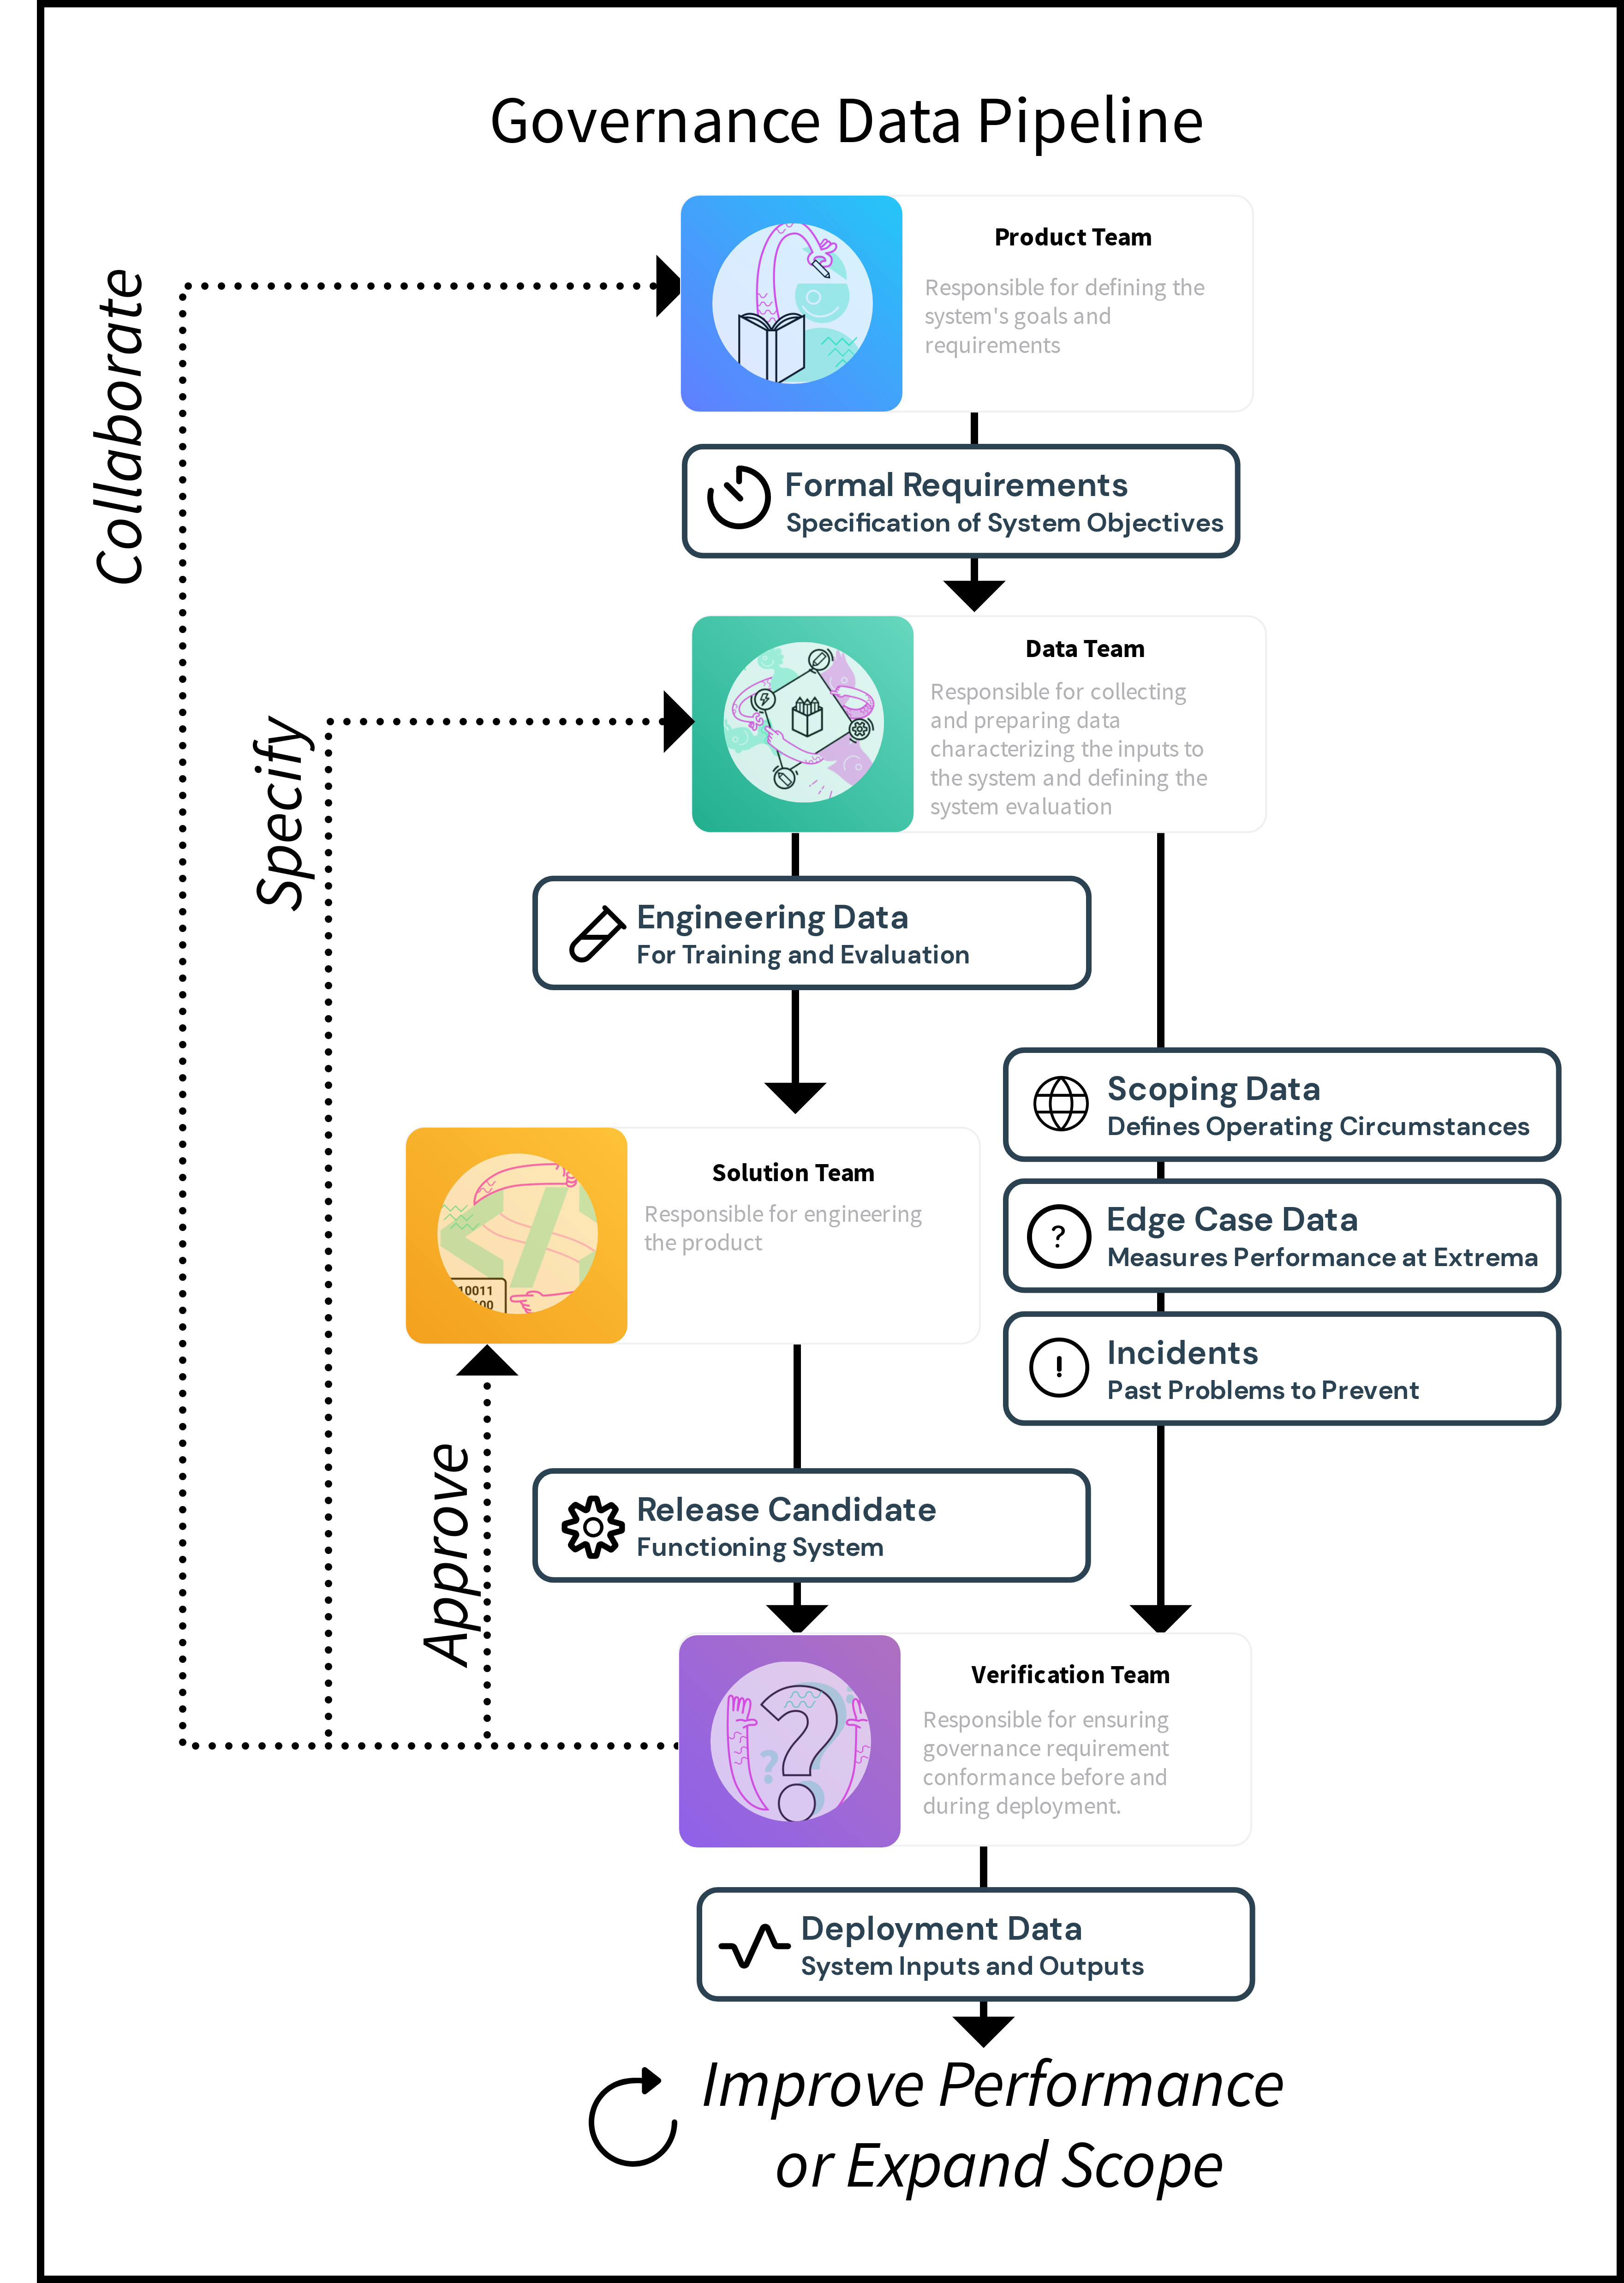
\includegraphics[width=0.80\textwidth]{images/PenpotPipeline.png}
    \caption{Teams and their interactions in the data production process. Every product begins its life with the product team defining the formal requirements for the solution in coordination with the verification team. The Data team then takes the requirements and collaborates with the Solution Team in the production of representative data. The Data Team's outputs are then either issued to the Solution Team or to the Verification Team, which subsequently takes delivery of the release candidate from the Solution Team. The verification team makes the final determination of whether the solution meets governance requirements before permitting its deployment. At the end of the process the development cycle is reentered to either improve system performance, or to expand the system scope via data now available.}
    \label{fig:data_pipeline}
\end{figure}

Defining scope and collecting edge cases are standard concepts in the safety engineering community, but their realization in AI systems, which are probabilistic, is distinctive. Without collecting the data according to the data engineering process of Figure \ref{fig:data_pipeline}, the capacity to know what the system will do is compromised and system governance is rendered impossible. Datasets consistent with Figure \ref{fig:venn} require careful construction where only the data team has a comprehensive view of the data space. Indeed, many large technology companies with vast stores of user data recognize these risks, and thus make the data available selectively to solution and analytics teams without fully exposing the non-aggregated data to those teams.

\begin{figure}[ht]
    \centering
    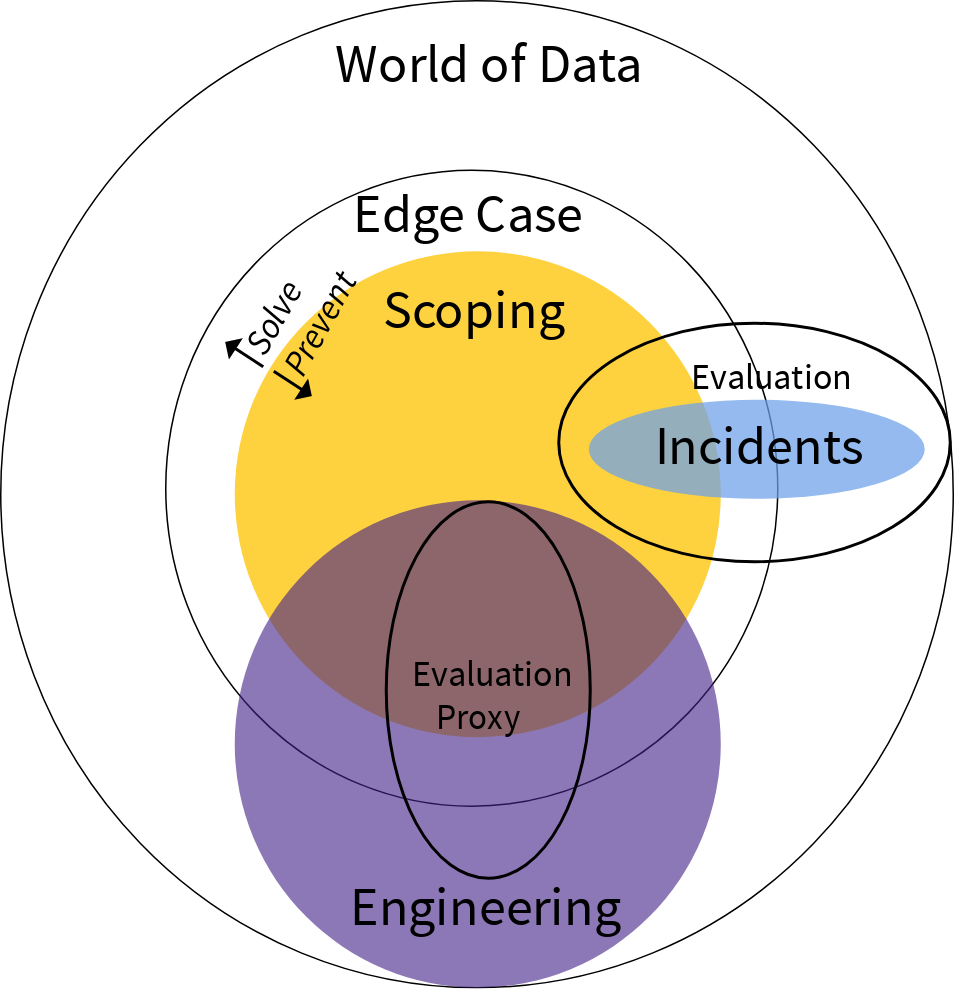
\includegraphics[width=0.4\textwidth]{images/PenpotVenn2.png}
    \caption{Relationships among the datasets discussed in this section. All data should be consistent with data that can occur within the system's deployment environment. The engineering data is available to the solution team to improve the performance of the system. The scoping data characterizes the operating envelope of the system and, thus, when the system is beyond its competencies. The edge case data defines challenging instances at the boundaries of the system's scope that require solutions. The incident data characterize instances where harms have occurred or nearly occurred as a result of the system. The incidents are not directly available to the engineering team, but they should be covered by the evaluation proxy, which is meant to mirror the true performance evaluation that encompasses all incidents and a sampling of the non-incident data space. }
    \label{fig:venn}
\end{figure}

% In the next section we shift from incidents as motivating data-centric governance to a higher level description of what constitutes data-centric governance.
